\documentclass{article}
\usepackage[utf8]{inputenc}

\title{TT3010 - Audio technology and room acoustics. \newline Exercise 6 - Music scales.}


%\author{Jan Arne Bosnes}
\date{\today}

\usepackage{natbib}
\usepackage{graphicx}
\usepackage{multicol}
\usepackage{gensymb}
\usepackage{float}
\usepackage{wasysym}


\begin{document}

\maketitle

All tasks are based on chapter 9 in Rossings "Science of Sound" \cite{rossing}. 
It is recommended that the student will try to do every task, but tasks marked \textit{Mandatory} are to be handed in for approval (online). Deadline is November 16 at 16:00.

\section*{Tasks}
%\begin{multicols}{2}
\begin{itemize}
    \item [1.] Verify by direct multiplication that a major third in equal temperament has the ratio of 1.26 and a minor third has the ratio of 1.19.
  
    \item[2.] From your knowledge of equal temperament, show that if you invest money at an interest rate of 5.9 \% compounded annually, your investment doubles  in 12 years.
    
    \item[3.] \textit{Mandatory} An octave-band sound analyzer measures the sound level in 10 octave bands with center frequencies 31.5, 63, 125, 250, 500, 1000, 2000, 4000, 8000, 16 000 Hz. What are the closest notes on the musical scale?

    \item[4.] \textit{Mandatory} The sound used in a touch-tone telephone have the following frequencies: 697, 770, 850, 941, 1209, 1337 and 1477 Hz. What are the closest notes on the musical scale?
    
    \item[5.] Verify by multiplication that a fifth plus a fourth equals an octave in any tuning, as does a major sixth plus a minor third.
    
   % \item[6.] (Not used) According to the data in Figure 7.2 the jnd in frequency up to about 700 Hz (roughly the lower half of the piano keyboard) is about 3 Hz. Convert $\delta f/f$ = 3/400 to cents. Then refer to table 9.2 (or figure 9.6) and answer the following.
    %\begin{itemize}
    %    \item[a.] Can one normally hear a difference between A4 on the just, Pythagorean, and tempered scales based or, C?
    %    \item[b.] How about E4, F4 and A4?
    %\end{itemize}
    
    \item[6.]  Using the frequency ratios given in figure 9.5, verify that the intervals C : G, E : B, F : C, G : D and A : E are perfect fifths in the just diatonic scale. Determine the frequency ratios for the imperfect fifth D : A. 

    \item[7.] \textit{Mandatory}  Find the frequency ratio that corresponds to 25 (cent). What are the frequencies of the note A4 + 25 (cent)? What about A4 - 25 (cent)?  
    
    \item[8.] \textit{Mandatory} Some tuning forks are designed to a scale which the C's have frequencies that are powers of 2 (128, 256, 512 Hz, etc.). How many cents flat are they compared to the international standard frequencies given in table 9.22?
    

\end{itemize}

%\end{multicols}

\begin{figure}[H]
    \centering
    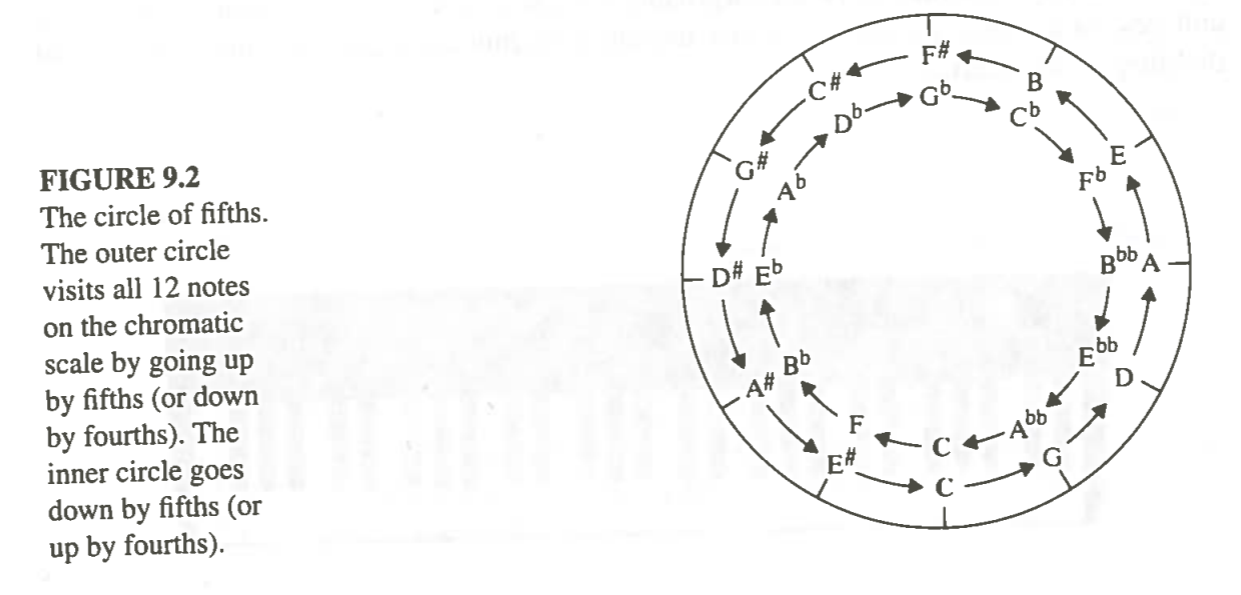
\includegraphics{figures/oving9_1.png}
    \label{fig:1}
\end{figure}

\begin{figure}[H]
    \centering
    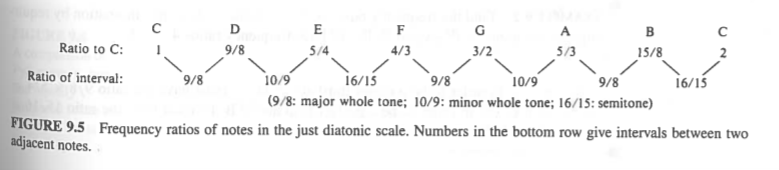
\includegraphics[scale=1.5]{figures/oving9_4.png}
\end{figure}

\begin{figure}[H]
    \centering
    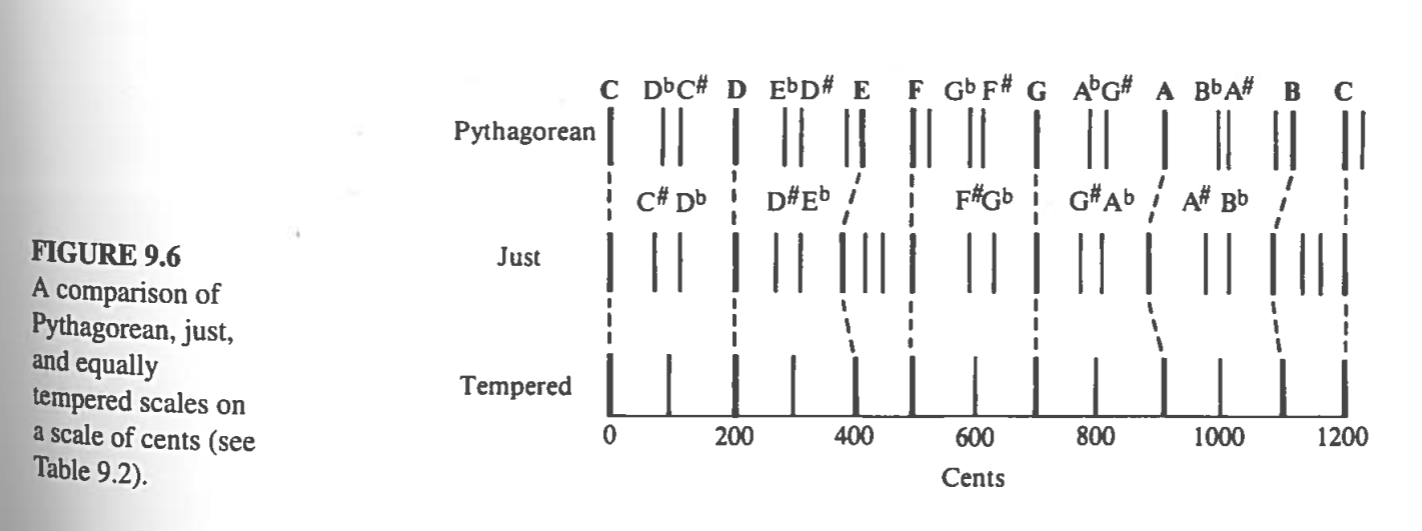
\includegraphics{figures/oving9_2.png}
    \label{fig:2}
\end{figure}

\begin{figure}[H]
    \centering
    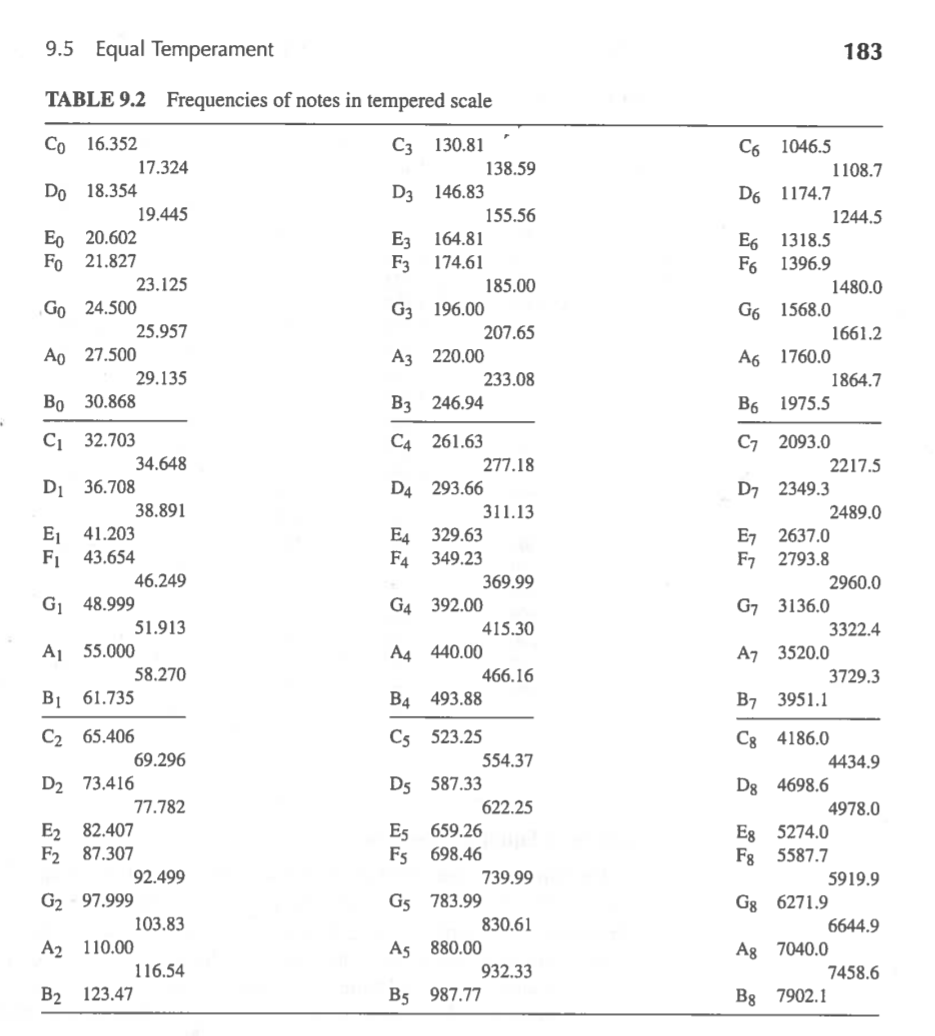
\includegraphics[scale=1.3]{figures/oving9_3.png}
    \label{fig:3}
\end{figure}

\end{document}

